\documentclass{article}
\usepackage{graphicx}
\usepackage{siunitx}
\usepackage{csvsimple}

    \begin{document}
        \section{Implementation of Flip-Flop D and SR Latch with discrete logic gates}
        Using the schematic on Figure \ref{fig:Schem} the logic gates were implemented on a PCB.
        
        \begin{figure}[h]
            \begin{center}
                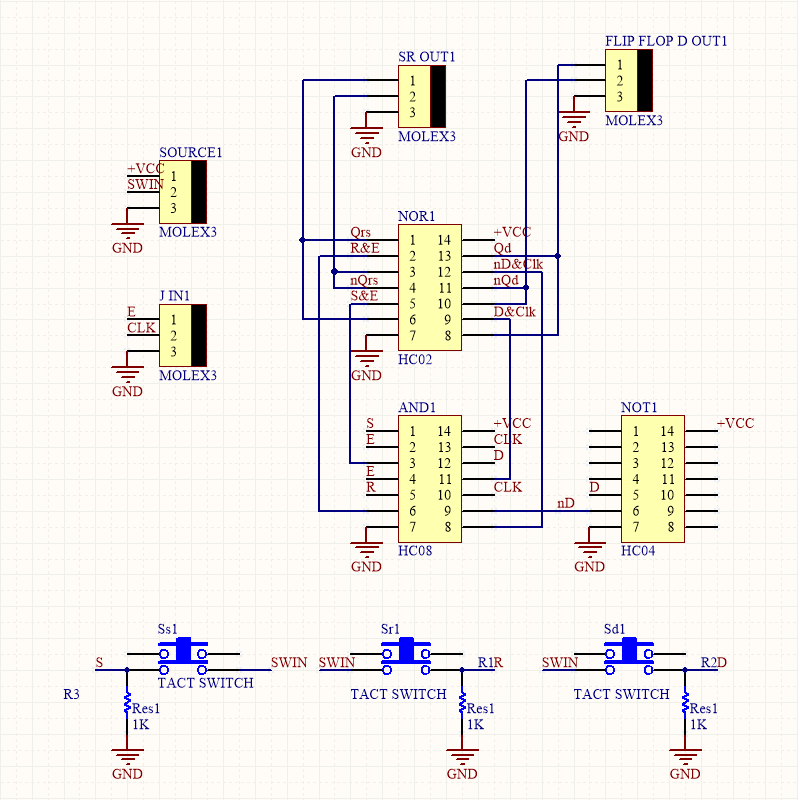
\includegraphics[width=\linewidth]{e6Schem.png}
                \caption{Schematic of the  SR Latch (on the left) and Flip-Flop D (on the right)}
            \end{center}
            \label{fig:Schem}
        \end{figure}

        The resulting circuits were tested and compared to their resulting counterparts as shown in Table \ref{tab:e6res}.
        \begin{table}
            \begin{center}
                
            \end{center}
            \label{tab:e6res}
        \end{table}
            


    \end{document}